\documentclass[a4paper,11pt,onecolumn]{article}
\usepackage[hscale=0.8,vscale=0.9]{geometry}
\usepackage[parfill]{parskip}
\usepackage{amsmath}
\usepackage{amsfonts}
\usepackage{graphicx}
\usepackage{subfigure}
\usepackage{wrapfig}
\usepackage{amssymb}

\newcommand{\eat}[1]{}

\begin{document}
\include{weld-defns}
\title{Open-domain Knowledge Extraction}
\author{Niranjan Balasubramanian}
\maketitle
\eat{
1 Introduction 1
1.1 Motivation . . . . . . . . . . . . . . . . . . . . . . . . . . . . . . . . . . . . . . . . . . . . 1
1.2 Research challenges . . . . . . . . . . . . . . . . . . . . . . . . . . . . . . . . . . . . . . . 2
1.3 Contributions . . . . . . . . . . . . . . . . . . . . . . . . . . . . . . . . . . . . . . . . . . 4
2 Background 4
2.1 Reducing network energy consumption . . . . . . . . . . . . . . . . . . . . . . . . . . . . 4
2.2 Reducing the energy consumption of other device components . . . . . . . . . . . . . . . . 5
3 Power management as a network primitive 5
3.1 Preliminary work . . . . . . . . . . . . . . . . . . . . . . . . . . . . . . . . . . . . . . . . 6
3.2 Proposed work . . . . . . . . . . . . . . . . . . . . . . . . . . . . . . . . . . . . . . . . . 8
3.2.1 System architecture . . . . . . . . . . . . . . . . . . . . . . . . . . . . . . . . . . . 8
3.2.2 Interfacing with mobile device components . . . . . . . . . . . . . . . . . . . . . . 9
3.2.3 Leveraging external devices . . . . . . . . . . . . . . . . . . . . . . . . . . . . . . 10
4 User-centric power management 11
4.1 Background . . . . . . . . . . . . . . . . . . . . . . . . . . . . . . . . . . . . . . . . . . . 11
4.2 Preliminary work . . . . . . . . . . . . . . . . . . . . . . . . . . . . . . . . . . . . . . . . 11
4.3 Proposed work . . . . . . . . . . . . . . . . . . . . . . . . . . . . . . . . . . . . . . . . . 12
4.3.1 Modeling energy consumption of a user . . . . . . . . . . . . . . . . . . . . . . . . 12
4.3.2 Leveraging user-activity prediction . . . . . . . . . . . . . . . . . . . . . . . . . . 13
5 Development Plan and Timeline 14
6 Broader Impact 14
7 Curriculum Development Activities 15
8 Prior NSF Support 15
9 Data Management Plan 16
}
\section{Introduction}

\subsection{Motivation}

Building systems that can understand and reason with information present in texts is a central pursuit in the AI vision. Extracting and understanding information in texts itself requires background knowledge. It is no surprise that documents written for human consumption assume background knowledge and an inference capability that reads between lines. For example, consider the following news snippet:

\begin{verbatim}
        Somalia's al-Shabab militant group has confirmed the death 
        of its leader in a U.S. airstrike and named his successor. 
        The al-Qaida linked militants announced the selection of 
        Abu Ubeid Ahmed Omar to replace Abdi Godane. 
\end{verbatim}

Reading these two sentences, we can easily conclude that {\em Abdi Godane} was the leader of {\em al-Shabab}, which is a {\em terrorist group} and {\em Abu Ubeid Ahmed Omar} is the successor of {\em Abdi Godane}, and {\em Abdi Godane} was killed by a {\em U.S.} airstrike. None of this information is explicitly mentioned in the sentences but can be {\em easily} inferred by humans. However, this inference is not so {\em easy} for extraction systems. 

Most information extraction systems target binary relations hat were explicitly mentioned in texts and cannot account for the implicit or inferred relations easily. Even within the explicitly expressed relations, many closed-domain IE systems can only extract a small set of manually pre-specified relations limiting their use to a small number of domains. On the other hand, Open IE systems extract every possible relation explicitly stated in text and do not have any notion of salience or importance to the main events in the discourse. Furthermore, binary relations do not capture the complexity of events that have multiple actors who perform specific roles within the event. 

To effectively address these issues, extraction systems need background knowledge that provide models or expectations for the information they need to extract. For example models of salient aspects of certain types of entities (e.g., actors {\em act in} movies, actors {\em win} awards) can help extract and organize information about people. Similarly, rich descriptions of events or scenarios, processes and their interactions can help in extracting and understanding information about events from texts. Scalable methods for acquiring such background knowledge is essential for building broad coverage extractors.

Template-driven extraction aims to address these issues by pre-specifying an extraction template for each event type (e.g., arrest, arson, bombing). The template describes an event type in terms of the actors and the roles they play within the event. Figure~\ref{fig:arrest} shows an example arrest template (or schema).  The key actors are an arresting agent who arrests and charges a suspect, a lawyer who represents the suspect and a judge who rules on the case. 
\begin{wrapfigure}{lh}{0.5\textwidth}
	\vspace{-2ex}
	\begin{center}
	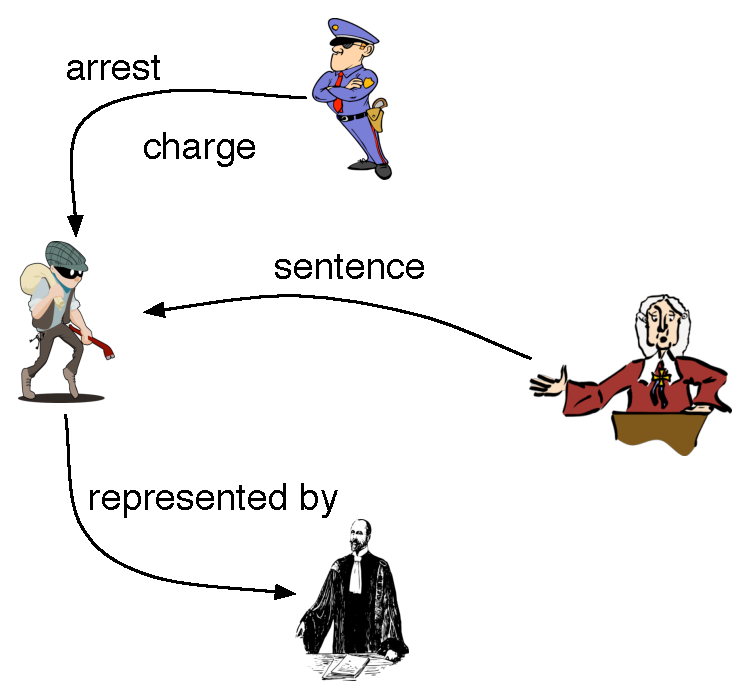
\includegraphics[width=2.5in,height=2in]{arrest-scenario} 	
	\vspace{-2ex}
	\caption{\label{fig:arrest} {\small Arrest schema: A model for an arrest scenario including key actors, the police, the suspect, judge etc. and their roles.}}
	\end{center}
\end{wrapfigure}
However, templates are fundamentally limited by the cost of manual authoring. Chambers and Jurafsky (2009) developed an automatic method for generating event schemas that scaled to arbitrary domains but used a simple representation that resulted in schemas that were mostly incoherent because they mixed distinct events (e.g., fire spreading vs. disease spreading). 

In this work, we target extraction of rich schemas that describe events using a range of information as shown in the table below.

\begin{table}[htdp]
\caption{default}
\begin{center}
\begin{tabular}{|p{4cm}|p{12cm}|}
\hline
Entities & Extractors\\
& Researcher, Organization, Subject, Problem, Conclusion, Publication, Date, Location \\
\hline
Sub-events &  \\
& R: Researcher study Problem (X)\\
& R find found/discovered/uncovered/stumbled/ Conclusion (Y) \\
& R published Results/Conclusions in [Journal/Book/Conference] \\
& R supports/refutes \\
& \\
\hline
Background-relations & \\
& R: Researcher, employed by, O:[Organization] \\
& study: Research, funded by, O:[Organization] \\
\hline
Entity Extractors & \\
& X:[Person] studies Y: [Problem] $\rightarrow$ X: [Researcher] \\
& X is studied by Y: [Person] $\rightarrow$ X: [Subject]\\
& X: [Researcher] concludes Y $\rightarrow$ Y: [Conclusion]\\
\hline
Relation Extractors & \\
	& study -- studied, investigated, explored, asked\\
	& find -- discovered, uncovered, stumbled \\			
\hline
Dependencies (Rel-grams) & \\
& R found Y, Conclusion(Y) $\rightarrow$ R publishes Y \\
& R found Y, Conclusion(Y) $\rightarrow$ R studied X \\	
\hline
Related Scripts & \\
& investigate, publish \\
\hline
\end{tabular}
\end{center}
\label{default}
\end{table}%


In preliminary work, we generated {\em coherent} event schemas for arbitrary domains. It leveraged the scalability of Open Information Extraction to produce a representation that included more context and used a simple generalization of the arguments to address sparsity. 

%These open-domain event schemas are but a starting point for aggregating and organizing background knowledge about events that can be leveraged during extraction. The main goal of this project is to build open-domain script like knowledge about events. 

Script-like knowledge serve as general purpose description of events or scenarios. In addition to the key actors, their actions, we will build scripts that include causal, temporal and dependency relationships between the different actions. During extraction this richer representation will enable us to infer more than what is explicitly mentioned in the text. 

Schemas provide a high precision model of scenarios which can be expanded to associated extractors -- i.e., patterns that can be used to extract from new texts. Resolving entity and event co-references. Third, scripts must include causal and temporal ordering of the actions in a scenario. 

\subsection{Research Challenges}



\subsection{Contributions}

\section{Background}

\section{Open-domain Background Knowledge Extraction}

\section{}





%The problem becomes worse when trying to extract information about events with multiple actors performing different roles. Template-driven extraction (Template IE) uses templates for event types (e.g., arrest, arson, bombing) and extract information into slots that correspond to actors and their roles. While templates provide a rich output structure, they are fundamentally limited by the cost of manual authoring of templates. Until recently there was no analog to Open IE for template IE. Chambers was the first to show how such templates can be automatically mined from text. However, the work resulted in schemas that mix events from different domains and with a small number of actors. In our previous work we enhanced schema generation by using an Open IE solution that scale to arbitrary domains but also resulted in highly coherent schemas with many actors. 
%Macro-reading works for accumulating factual statements: e.g., nationality(Maradona, Argentina), player(Maradona, Soccer) etc. However, micro-reading is often essential to answering questions about individuals or events that are not discussed often in texts. For example, consider a snippet from a news article:



For example,
..\\
..\\
..\\

Even news stories written by journalists trained to produce self-contained articles assume common-sense and inference capabilities that are far beyond existing information extraction capabilities. For example, 
..\\
..\\
..\\

The goal of this project is to investigate corpus-driven approaches for mining background knowledge. In particular, we will investigate approaches that aggregate and connect frequently co-mentioned fact mentions into structured representations of generalized knowledge. For example, 

..\\
..\\
..\\

The project will proceed in three phases:
\begin{itemize}
\item Knowledge Representation


Identify and design a suitable representation for the background knowledge by analyzing manually generated background knowledge. The idea here is to design games that help elicit readers to specify the background knowledge they use in reading or understanding a document. 
Once we have aggregated the various forms of knowledge we will design a suitable representation that allows for . 

\item Extraction and Generalization -- In this phase we will 

\item Aggregation and Consolidation


\end{itemize}

\section{Knowledge Representation}

\section{Acquisition and Generalization}

\section{Aggregation and Consolidation}

\section{Development Plan and Timeline}

The project will proceed in three phases. In the first phase of the project, we focus on the designing the representation and extracting information from large corpora using existing IE systems. We will design a rich representation for the targeted knowledge by leveraging existing ontologies for entities and relations (e.g., YAGO, NELL, Freeebase) where possible and using text derived representations in other places. Then, we will investigate techniques for aggregating and generalizing information in the specific instances. In particular, we will develop automatic methods for choosing the right level for mapping into a type hierarchy for the arguments and the relations. In the second phase, we will focus on graph-based approaches for generating open-domain schemas using the generalized extractions. In our preliminary work, we identified the graph properties that indicate specific characteristics for good schemas and developed a suitable method that exploited the graph properties to produce high-quality schemas. In the third phase, we will focus on applying the generated schemas to two end tasks: event extraction, and summarization. For event extraction we will build extractors. Schemas can be thought of as high-precision models of events, which can then be expanded to include higher-recall extractors via bootstrapping. For summarization, we will use schemas to help select sentences for the standard MUC single document summarization task. We will iterate and refine the schema representation and generation based on their performance in these end tasks.

Year 1:  
\begin{enumerate}
\item Design target Representation for Knowledge  Design representation manually based on use cases from target applications.
\item Information Extraction and Aggregating existing knowledge. Annotate documents using Open IE and link entities to existing resources. Explore Generalization Techniques 
� Develop methods for generalize specific instances (e.g., John was arrested in Bristol, UK �> [Person] arrested in [Location])
\item Construct micro-theories using corpus analysis. Co-mentioned (and argument sharing) instances are likely part of some theory. Mechanical Turk Evaluation of Micro-Theories.
\end{enumerate}

Year 2:
\begin{enumerate}
\item Relate micro-theories to each other 
\item Inference over graphs to enhance recall and precision of theories..
\item Iterative development w/ target application: 1) Apply learned theories to target application. 2) Recall is often an issue. Explore on demand construction of theory given a particular document. 
\end{enumerate}


\section{Broader Impact}

Event schemas directly impact many practical applications and provide a stepping stone for advances in knowledge-intensive AI applications. Businesses gather ever increasing amounts of data from customers and users via social platforms, analysts deal with increasing news volumes, researchers produce and consume vast amounts of knowledge through publications. All these diverse communities can benefit from scalable information extraction and summarization systems. Event schemas are an important step towards automatically building script-like knowledge from text, which can benefit knowledge-intensive AI applications such as reasoning and Question Answering. Furthermore, the method and techniques can scale to other domains and spur research on similar problems (e.g., extracting processes from textbooks, identifying schemas in research studies).

\section{Curriculum Development Activities}

I plan to teach a course centered around the core concepts of scalable information extraction and knowledge extraction techniques. 
Most technology companies with a large web presence have a need for extracting information of one form or other from information obtained by engaging with their user base. This course will provide a basic overview of a distributed information extraction pipeline, persistence, and building applications that rely on the extracted data. 

\section{Prior NSF Support}

\section{Data Management Plan}
 
{\small
\bibliographystyle{plain}
\bibliography{../research-statement,../kia}
}
\end{document}
